% LaTeX file for Chapter 02


\chapter{Methods} 

\section{DEXSeq}
DEXSeq \citep{dexseq} is a statistical method originally proposed to test for differential exon usage in RNA- seq data, which has been widely adopted in other contexts too, such as differential transcript usage \citep{swimming_downstream}. The model is based on the negative binomial distribution and allows for covariates such as batch effects to be taken into account to offer reliable control of false discoveries \citep{dexseq}. In its original implementation DEXSeq inputs how many reads map to each exon, but the method has alsob been used on transcript level counts. Equation (\ref{eqn:DEXSEQ_A}) shows that the read counts follow a negative binomial distribution where $\alpha$ is the dispersion parameter. Further, a generalized linear model is used to predict the mean via a log-linear link:

\begin{equation}
K_{ijl} \sim \text{NB}(\text{mean}=s_j \mu_{ijl}, \text{dispersion}=\alpha_{il})
\label{eqn:DEXSEQ_A}
\end{equation}

\begin{equation}
log(\mu_{ijl}) = \beta^G_i + \beta^E_{il} + \beta_{i \rho_j}^C + \beta^{EC}_{i \rho_j l}
\label{eqn:DEXSEQ_B}
\end{equation}

where $\text{NB(a, b)}$ denotes the negative binomial distribution with mean a and dispersion b, $s_j$ is .. \\

The dispersion parameter allows to model over-dispersed data (i.e. higher variance than mean). Here, we propose to use DEXSeq on estimated USA counts, and perform a differential usage test between conditions. This models ambiguous reads separately from spliced and unspliced or exonic and intronic, thus eliminating one of the main sources of mapping uncertainty. However, the uncertainty related to reads mapping to multiple genes is still neglected by this approach.

\section{minnow}
\emph{minnow} is a read level simulator for droplet based scRNA-seq data that accounts for important sequence-level characteristics and model effects \citep{minnow}. It matches the gene-level ambiguity characteristics that are present in real scRNA-seq experiments. With \emph{minnow} it is possible to demonstrate the effect of gene-level sequence ambiguity on accurate quantification, which is used in this thesis to simulate mapping uncertainty between spliced and unspliced counts. It achieves this by simulating the reads by sampling from the underlying reference transcriptome.

\section{Classification measurements}
The TPR, FPR, and FDR are defined as:

\begin{equation}
\text{TPR}=\frac{|\text{TP}|}{|\text{TP}+\text{FN}|}
\label{eqn:tpr}
\end{equation}

\begin{equation}
\text{FPR}=\frac{|\text{FP}|}{|\text{FP}+\text{TN}|}
\label{eqn:fpr}
\end{equation}

\begin{equation}
\text{FDR}=\frac{|\text{FP}|}{|\text{TP}+\text{FP}|}
\label{eqn:fdr}
\end{equation}

where TP, TN, FP, and FN indicate the sets of true positive, true negative, false positive, and false negative elements, respectively. True positive (TP) are the number of elements that were correctly identified as the positive outcome. Similarly, true negative (TN) are the number of elements that were correctly identified as the negative outcome. False positive (FP) are those elements that were identified as the positive outcome, however they should have been identified as negative. In statistics, FP is usually referred to as Type 1 error. Similarly, false negative (FN) are the elements that were incorrectly identified as negative - also referred to as Type 2 error in the realms of statistics. Figure \ref{fig:confusion_matrix} illustrates the meaning of these measurements quite clearly. The TPR (true positive rate) also referred to as sensitivity, measures the proportion of positive elements that were correctly identified - often alluded to as statistical power \ref{eqn:tpr}. The FPR (false positive rate) measures the proportion of negative outcomes that are identified as positive \ref{eqn:fpr}. On the other hand, FDR (false discovery rate) measures the expected proportion of false positive among all positive predictions \ref{eqn:fdr}. 

\begin{figure}[!htb]
\begin{center}
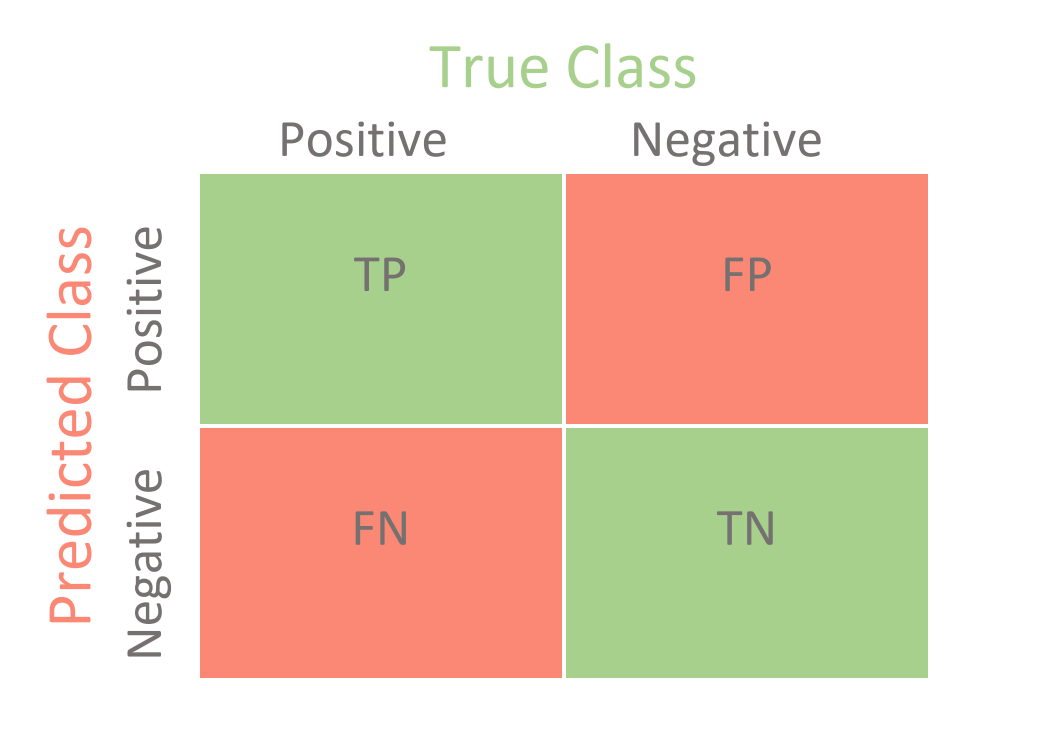
\includegraphics[width=6in,height=4in]{figure/confusion_matrix.png}
\end{center}
\caption{Confusion matrix reporting the performance of a binary classification problem}
\label{fig:confusion_matrix}
\end{figure}
\FloatBarrier

\section{ROC curve}
The ROC curve is a performance measurement that is used for classification problems - in this case whether a gene is differently expressed or not. Essentially, the ROC curve is a probability curve that is plotted with TPR against the FPR where TPR is on the y-axis and FPR on the x-axis. ROC curves above the diagonal are considered helpful, where the diagonal line represents random guessing. ROC curves are one of the performance evaluation methods used in this thesis.

\section{TPR v. FDR curves}
The TPR v. FDR curves are usually evaluated at typical thresholds of nominal 1\%, 5\% and 10\%. When the observed FDR is lower than or equal to the specified threshold, the method controls for the FDR. However, if the observed FDR is greater than the threshold the method does not control for the FDR and there is an inflation of false positive predictions. In this thesis, the methods are evaluated by an adjusted p-value.

\section{Differential regulation}
To address both sources of mapping uncertainty we propose our novel method. Similar to the idea above, we implemented a hierarchical Bayesian approach that models ambiguous counts separately from spliced and unspliced. Gene allocation is modeled as a latent state to address the gene-related mapping uncertainty. The model consists of two nested models: First, we use a Dirichlet-multinomial model for the relative abundance of the USA counts in each gene. Second, a multinomial model that models the relative abundance of genes for each sample individually.

